\documentclass[journal]{IEEEtran}
\usepackage{amsmath,amsfonts}
\usepackage{algorithm,algpseudocode}
\usepackage{array}
\usepackage[caption=false,font=normalsize,labelfont=sf,textfont=sf]{subfig}
\usepackage{textcomp}
\usepackage{stfloats}
\usepackage{url}
\usepackage{verbatim}
\usepackage{graphicx}
\usepackage{listings}
\usepackage[bookmarksnumbered, colorlinks, plainpages]{hyperref}
\usepackage[dvipsnames]{xcolor}
%\hyphenation{op-tical net-works semi-conduc-tor IEEE-Xplore}
\usepackage{balance}
\newcount\myloopcounter

\definecolor{codegreen}{rgb}{0,0.6,0}
\definecolor{codegray}{rgb}{0.5,0.5,0.5}
\definecolor{codepurple}{rgb}{0.58,0,0.82}
\definecolor{backcolour}{rgb}{0.95,0.95,0.92}

\lstdefinestyle{mystyle}{
    backgroundcolor=\color{backcolour},   
    commentstyle=\color{codegreen},
    keywordstyle=\color{magenta},
    numberstyle=\tiny\color{codegray},
    stringstyle=\color{codepurple},
    basicstyle=\ttfamily\footnotesize,
    breakatwhitespace=false,         
    breaklines=true,                 
    captionpos=b,                    
    keepspaces=true,                 
    numbers=left,                    
    numbersep=5pt,                  
    showspaces=false,                
    showstringspaces=false,
    showtabs=false,                  
    tabsize=2
}
\lstset{style=mystyle}

\newcommand{\repeatit}[2][10]{%
  \myloopcounter0% initialize the loop counter
  \loop\ifnum\myloopcounter < #1 % Test if the loop counter is < #1
  #2%
  \advance\myloopcounter by 1 % 
  \repeat % start again
}

\begin{document}
\title{Final Report of the Group Project for CS5351\\
\colorbox{yellow}{\textit{!We Need Project Title: An informative title!}}
}

\input{private/author}


%\markboth{Journal of \LaTeX\ Class Files,~Vol.~18, No.~9, September~2020}%
%{How to Use the IEEEtran \LaTeX \ Templates}

\markboth{Final Report of the Group Project for CS5351, December~2023}%
{Title of the Project TBD.}

\maketitle

\begin{abstract}
This document describes blablabal....
abstract to be consideration.

\textit{Requirements: needs (150 words) }

\end{abstract}

\begin{IEEEkeywords}
Software Engineering, Software Testing, Computer Science, Software Maintainance, Software Debug.
\end{IEEEkeywords}


\section{Introduction}
\IEEEPARstart{I}{n} rapidly developing society, information technology has made significant advancements and has gradually become deeply ingrained in every aspect of people's lives. It plays a crucial role in various aspects of people's lives. Simultaneously, an increasing number of individuals are trusting the security of network technology and entrusting more of their private information to the internet. Since privacy exists, it is inevitable that there will be malicious users who, for various reasons, attempt to invade privacy, also known as threat actors. Web applications, due to their short development cycles and developers' inadequate security awareness, often contain various vulnerabilities. Malicious users exploit these vulnerabilities in web applications to gain valuable information and pose a threat to users and businesses.

In this context, it can be observed that many information security issues stem from code-related problems. According to Gartner, the leading global IT research and consulting firm, nearly 75\% of hacking incidents are related to system code security. Product developers may create security risks due to a lack of sufficient knowledge about information security while writing code. Insecure code not only becomes exploitable but can also assist malicious users. Therefore, before a product is launched, code auditing, which provides security guarantees, is essential. Code auditing involves reading and examination of source code by auditors to identify potential security vulnerabilities or coding irregularities, highlighting code defects that may lead to security loopholes, and providing recommendations for modifications in the audit report. Conducting thorough code audits is a cost-effective way to ensure product security and a timely approach to discovering vulnerabilities, thereby enabling proactive prevention of potential attacks. Effective code security auditing can significantly reduce the security risks of software, minimizing the need for subsequent remedial work such as security assessments, reinforcements, controls, and maintenance. It transforms passive intrusion protection into proactive defense against vulnerabilities in products. Secure and stable products contribute to the sustained efficient operation and development of businesses.

Automated code auditing methods differ from manual auditing. They offer high efficiency and increased speed in auditing source code. They reduce the professional requirements for auditors, making it easier for beginners to operate and generate reports. Moreover, automated auditing provides a completely objective perspective, comprehensively auditing all source code, preventing auditors from being influenced by developers and unable to engage in independent thinking and judgment. It also helps identify weak functional code that can easily be overlooked in manual auditing, which may pose security vulnerabilities and threaten the security of individuals and businesses' data.

Web automation testing tools are tools used for automating the testing and detection of security vulnerabilities in web applications. They assist developers and security professionals in identifying and fixing common security vulnerabilities in web pages, such as SQL injection and DNS poisoning. With the increasing awareness of network security, more organizations and developers have begun to pay attention to and prioritize the security of web applications. They aim to promptly identify potential security vulnerabilities and take appropriate measures to rectify and prevent them. Web automation testing tools aid developers in conducting preliminary security testing on web pages through automation, providing accurate security assessment results. Traditional security testing typically requires significant human resources and time investment, involving manual penetration testing and vulnerability scanning, which fails to meet the demands of rapid iteration and continuous delivery. Web automation testing tools offer an automated solution that significantly reduces testing time and workload, thereby improving testing efficiency and accuracy. They assist organizations in ensuring data confidentiality and integrity by conducting security testing and addressing security vulnerabilities.

\section{Related Work}
\noindent Web security has become quite important nowdays due to the increase in cybercrimes. Developers are very concerned about how to avoid obvious security issues such as hacking and data breaches, when designing and developing websites. There have been many studies that have proposed many technologies and tools to prevent web security vulnerabilities and defense methods, and there have also been many studies that have evaluated the effectiveness and missed detection probability of existing vulnerability scanning methods. 

Abirami's team created a tool to detect vulnerabilities such as XSS and SQLI using Python language. The program run automatically to send reports to relevant users\cite{9155908}. Zhang's team proposed an automatic detection tool dealing with multiple type of vulnerabilities. The tool includes a combination of three vulnerability detections, including cross-site scripting attacks, SQL injections, and directory operations\cite{8983828}. A web program named Gregorius used AJAX crawling to improve vulnerability detection efficiency\cite{9092613}. There is also a detector named ETSS, which is a versatile and modular online vulnerability detection created by Rocha and Souto that automatically checks web applications for XSS vulnerabilities. It can find and evaluate all data entry points of an application, as well as create code injection tests for each test\cite{6924244}. Web application penetration testing is designed to evaluate the design, configuration, and architecture of a web application. Shebli's group  studied penetration testing processes and tools, focusing on comparing four different port scanning tools to demonstrate their effectiveness\cite{8378035}. In recent years, with the development of machine learning, many web application vulnerability detection methods based on machine learning have emerged. Combined with the development history of machine learning security vulnerability detection technology, Lilan Hu's team designed and implemented a cross-site scripting security vulnerability detection model for web applications, a verification code identification function was added\cite{article10.1088/1742-6596/1827/1/012061}. Calzavara's group proposed a methodology to leverage machine learning for the detection of web application vulnerabilities. They used it in the design of Mitch, the first ML solution for the black-box detection of cross-site request forgery vulnerabilities\cite{8966601}.

\subsection*{Code Audit Tools}

The development history of code auditing techniques is relatively short, resulting in many security issues that should have been discovered during the development phase appearing in the deployed applications. This is particularly true for applications developed by small and medium-sized enterprises, where the emphasis is primarily on functionality, marketability, and design, with the code's security standards relying largely on the developers' awareness of security. The research on the process of code security auditing has primarily focused on classical programming languages such as C/C++. Software vulnerability detection techniques can be classified into three categories: static, dynamic, and hybrid. The code detection module in this project belongs to the category of static detection based on vulnerability rules.

According to a research in 2018,they leveraged the wealth of C and C++ open-source code available to develop a large-scale function-level vulnerability detection system using machine learning. Evaluate the tool on code from both real software packages and the NIST SATE IV benchmark dataset\cite{8614145}. The main idea of this research is beginning with designing a C/C++ lexical analyzer to capture the meaning of key words, while ensuring the universality of the representation and minimizing the total number of words. Then the data is processed and integrated, and labeled according to whether there is a vulnerability. Finally, the training results of the machine learning model show that deep feature representation learning on source code is a promising approach for automated software vulnerability detection.

Another research in 2011 focused on a different method. To reduce the redundancy of information in software static analysis and improve the accuracy and efficiency of the information extraction, a syntax trees model based on relational storage mode is proposed. Using the mature parsing technique on XML, a new static detection method based on XML model is put forward and applied to program norm\cite{5997729}. Their result shows that the method not only improves the detection efficiency but also increases the detection accuracy.

\section{Preliminaries}
\noindent The Preliminaries section lays the foundation for the reader by presenting essential technical background information. It encompasses a summary of the knowledge required to understand the developed tools, focusing on code smells, their significance, and existing tools in the domain. This section aims to equip the reader with the necessary context to comprehend the subsequent discussion.

\subsection{Vulnerability principle analysis}
Both manual code auditing and the process of designing and implementing automated code auditing systems require a proficient understanding of common vulnerability principles and manifestations, as well as a solid grasp of code patterns that may give rise to such vulnerabilities. When auditors examine source code, their knowledge of vulnerability-related concepts enables them to swiftly and accurately identify defective code and annotate it accordingly. In the case of designing automated code auditing systems, it is imperative to construct a rule library based on the pertinent knowledge of common vulnerabilities. This rule library should possess precise matching capabilities and high coverage, facilitating the accurate automated identification of code that may constitute security vulnerabilities.

The table \ref{tab:vulnerabilities} summarizes some commonly encountered vulnerabilities with elevated security threats. These vulnerabilities encompass, but are not limited to, the OWASP TOP 10 (Open Web Application Security Project)\cite{OWASPtop102017}, CVE (Common Vulnerabilities \& Exposures), PCI security standards, SANS20 (SysAdmin, Audit, Network, Security), and CWE (Common Weakness Enumeration) as disseminated by authoritative organizations in the field of security.

\begin{table}[h]
  \caption{vulnerabilities with high security threats}
  \label{tab:vulnerabilities}
  \begin{tabular}{p{0.4\linewidth}|p{0.5\linewidth}}
  \hline\textbf{Vulnerability}             & \textbf{Impact}                                          \\\hline
  Cross-Site Scripting (XSS)         & Phishing, identity theft, etc.                           \\\hline
  SQL Injection                      & Information disclosure, webpage tampering, etc.          \\\hline
  Server-Side Request Forgery (SSRF) & Unauthorized access, etc.                                \\\hline
  Remote Code Execution (RCE)        & Information disclosure, etc.                             \\\hline
  URL Redirection Vulnerability      & Phishing website deception, information disclosure, etc. \\\hline
  Variable Overwrite                 & Overwriting arbitrary database configurations           
  \end{tabular}
  \end{table}

\subsection{SQL Injection}
SQL Injection is a security vulnerability where untrusted user input is improperly handled or concatenated into SQL queries, leading to the execution of unintended SQL commands. Attackers can manipulate input to modify the query's structure, bypass authentication, or retrieve sensitive information from the database. This occurs due to the failure of input validation and the lack of parameterized queries or prepared statements, which allow user input to be treated as data rather than executable code.

\begin{lstlisting}[caption={PHP code SQL Injection},label={lst:sqlinjectphp},
  language=PHP,breaklines=true]
$username = $_POST['username'];
$password = $_POST['password'];
$query = "SELECT * FROM users WHERE username = '" . $username . "' AND password = '" . $password . "'";
\end{lstlisting}

In this piece of PHP code \ref{lst:sqlinjectphp}, if the parameters which in \verb|$_POST['username']| or \verb|$_POST['password']| are not properly validated or sanitized, an attacker can input malicious SQL statements as the values, thereby altering the intended SQL query structure and potentially gaining unauthorized access to the database.

\subsection{Cross-Site Scripting (XSS)}
Cross-Site Scripting is a vulnerability that occurs when untrusted user input is not properly sanitized or encoded before being displayed on a web page. This allows attackers to inject and execute malicious scripts within the victim's browser, leading to various attacks such as session hijacking, defacement, or data theft. 

\begin{figure}[h]
  \centering
  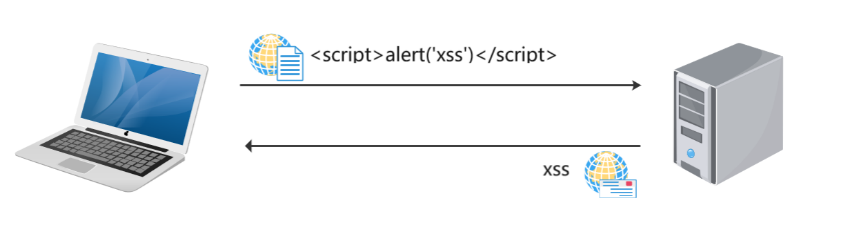
\includegraphics[width=3in]{figures/xss.png}
  \caption{Cross-Site Scripting (XSS)}
  \label{fig:xss}
  \end{figure}

XSS vulnerabilities typically arise due to the lack of input validation and output encoding when displaying user-generated content. It often caused by unqualified JavaScript code.

\begin{lstlisting}[caption={JavaScript Cross-Site Scripting (XSS)},label={lst:jsxss},language=HTML,breaklines=true]
var name = document.getElementById('name').value;
document.write("Welcome, " + name);
\end{lstlisting}

In this JavaScript example shown in \ref{lst:jsxss}, if the name value is not sanitized or encoded before being displayed using \verb|document.write()|, an attacker can inject JavaScript code as the value of name, leading to the execution of the injected script in the victim's browser.

\subsection{Server-Side Request Forgery (SSRF)}
Server-Side Request Forgery is a vulnerability where an attacker can manipulate a server's behavior by tricking it into making unintended or unauthorized requests to internal or external resources. This can lead to unauthorized access to sensitive information, port scanning, or even remote code execution. SSRF vulnerabilities typically occur when user-controlled input is used to construct URLs or make network requests without proper validation and access control.

\begin{lstlisting}[caption={Java Server-Side Request Forgery (SSRF)},label={lst:javassrf},language=JAVA,breaklines=true]
URL url = new URL(request.getParameter("url"));
HttpURLConnection connection = (HttpURLConnection) url.openConnection();
\end{lstlisting}

In the above Java code snippet in \ref{lst:javassrf}, if the user-provided url parameter is not properly validated or restricted, an attacker can supply a malicious URL that points to internal network resources, leading to SSRF.

\subsection{Remote Code Execution (RCE)}
Remote Code Execution is a severe vulnerability where an attacker can execute arbitrary code on a target system, potentially gaining full control over it. RCE vulnerabilities typically arise due to insecure coding practices, such as using user input directly in functions or commands without proper validation or sanitization. Attackers can exploit these vulnerabilities to run arbitrary commands, upload malicious files, or execute arbitrary code on the server.

\begin{lstlisting}[caption={PHP Remote Code Execution (RCE)},label={lst:phprce},language=PHP,breaklines=true]
$command = $_GET['command'];
exec($command);
\end{lstlisting}

In this PHP example in \ref{lst:phprce}, if the \verb|$_GET['command']| parameter is not properly validated or sanitized, an attacker can inject malicious commands, which will be executed by the exec() function, leading to arbitrary code execution on the server.

\subsection{URL Redirection}
URL Redirection vulnerabilities occur when untrusted user input is used to redirect users to unintended or malicious websites. Attackers can abuse this vulnerability to conduct phishing attacks, redirect users to malware distribution sites, or trick them into visiting unauthorized pages. This vulnerability arises when user-controlled input is directly used to construct redirect URLs without proper validation and sanitization.

\begin{lstlisting}[caption={Java URL Redirection},label={lst:javaurldr},language=JAVA,breaklines=true]
String redirectUrl = request.getParameter("redirect");
response.sendRedirect(redirectUrl);
\end{lstlisting}

In the above Java code in \ref{lst:javaurldr}, if the redirect parameter is not properly validated or restricted, an attacker can supply a malicious URL as the value, leading to unauthorized redirection of users to potentially harmful websites.

\subsection{Variable Overwriting}
Variable Overwriting vulnerabilities occur when the value of a variable can be controlled by an attacker, resulting in unexpected behavior or security issues in the code. This can happen due to insecure coding practices, such as allowing user input to directly modify critical variables without proper validation or sanitization, leading to unintended consequences or security breaches.

\begin{lstlisting}[caption={JavaScript Variable Overwriting},label={lst:jsvo},language=HTML,breaklines=true]
var isAdmin = false;
// Attacker-controlled input
isAdmin = true;
\end{lstlisting}

In this JavaScript example in \ref{lst:jsvo}, if the value of \verb|isAdmin| is influenced by user input without proper validation or access control, an attacker can overwrite the value of \verb|isAdmin| to true, potentially granting unauthorized administrative privileges.

\subsection{DNS poisoning}
DNS poisoning is a malicious attack aimed at disrupting the normal operation of the Domain Name System (DNS), which translates domain names to IP addresses. The principle behind DNS poisoning involves the manipulation of DNS responses to provide users with incorrect IP address or domain name mappings.
DNS poisoning can be categorized into two common attack methods: DNS cache poisoning and DNS hijacking.

\subsubsection{DNS cache poisoning}
In DNS cache poisoning, the attacker attempts to deceive recursive DNS servers into storing malicious DNS responses in their cache, which will be served to other users in subsequent queries, providing them with incorrect resolution results. The attacker sends DNS responses containing false IP address and domain name mappings, which may be mistaken as legitimate responses by recursive DNS servers and stored in their cache. When other users query the same domain, the recursive DNS server returns the cached incorrect response, redirecting the users to the wrong destination.

\subsubsection{DNS hijacking}
In DNS hijacking, the attacker attempts to intercept users' DNS requests and provide malicious DNS responses. The attacker may implement DNS hijacking through various means, such as setting up malicious DNS servers in infected routers or local networks or modifying DNS settings on users' devices through malicious software. When a user sends a DNS request, the attacker's malicious DNS server returns false IP address and domain name mappings, redirecting the user to a malicious website or server controlled by the attacker.

\subsection{Separation of front and back ends}
Front-end and back-end separation is a modern web development architecture, as shown in Fig.\ref{fig:Separation}, and design pattern that separates the front-end interface of the web page from the back-end server application logic, enhancing the maintainability of the application. Since front-end and back-end are independent, we can choose the technology stack that best suits our respective needs. For example, the front-end can use React, Vue.js or Angular, while the back-end can use Node.js, Python's Flask or Django, Ruby on Rails, etc. This separation improves development efficiency because development teams can independently update and extend different parts of the application without interfering with each other.

\begin{figure}[h]
  \centering
  
\includegraphics[width=2.5in]{figures/Preliminaries1.png}
  \caption{Separation of Front and Back ends}
  \label{fig:Separation}
  \end{figure}

\subsection{React for Front-End Development }
React is an open source JavaScript library widely used for building user interfaces. It allows developers to build applications using a componentized approach, meaning that each part of the user interface is encapsulated into independent, reusable components. React's responsive design principles ensure that the user interface can quickly respond to data changes. Fetch API is used for network requests in React applications. In this project, Fetch is used to communicate with the backend service to retrieve and send data.

\subsection{Ant Design of React}
Antd is a React UI library that follows the Ant Design specification and contains a set of high-quality components and demos for building rich interactive user interfaces.

\subsection{Cross-origin resource sharing}
Cross-origin resource sharing (CORS) is a security mechanism that allows or restricts resources on a web page (such as fonts, JavaScript, etc.) to be accessed by another domain name with a different origin. In the integration of React and Flask, CORS is an important consideration because the frontend and backend are usually deployed on different domains. Corresponding CORS strategies are used in this project to ensure safe and effective front-end and back-end communication.

\subsection{Postman}
Postman is an ideal tool for building and testing APIs. It supports all common HTTP request types, such as GET, POST, PUT, DELETE, etc. It allows users to easily add request parameters, header information, authentication data, etc. Postman provides a user-friendly interface that allows developers to easily send requests to the server and view the responses. By viewing the response data and status codes of the API, developers can quickly locate the problem.

\subsection{Flask for Back-End Development}
Flask is a lightweight web application framework written in Python. It is designed to be easily extensible and provides the necessary tools and features to build reliable web applications. In this project, Flask serves as the back-end framework to handle client requests and interact with the database.

\subsection{Database storage}
This project uses a database to store application data, which may include user information, transaction data, etc. In addition, the system supports file upload functionality, which is crucial for processing user-submitted code files. Flask provides integration with databases and the ability to handle file uploads.

\subsection{Nginx}
Nginx is a high-performance HTTP and reverse proxy server, which can also be used as a mail proxy server. In this project, Nginx is used as the web server, responsible for handling HTTP requests and forwarding them to the Flask application. The use of Nginx improves the reliability and load balancing capabilities of the application.

\subsection{Docker}
Docker is a popular open source containerization platform that allows developers to easily create, deploy, and run applications. By using Docker, developers can package applications and their dependencies into a portable container that can run on any Docker-enabled machine, ensuring application consistency across different environments.

\subsection{Kubernetes}
Kubernetes, also known as K8s, is an open-source container orchestration platform designed to automate the deployment, scaling, and management of containerized applications.  Kubernetes groups containers into logical units called pods, facilitating seamless management and discovery. Its core features include automated scaling, pod orchestration, services for networking, replication controllers, and deployments for ensuring application stability. With a master-node architecture, extensibility through Custom Resource Definitions (CRDs), and a vibrant community, Kubernetes has emerged as the industry standard, streamlining the complexities of containerized application deployment and management.


\section{Solution}
\noindent The Solution section articulates the team's approach to addressing code smells using an innovative tool. This part of the report encompasses detailed descriptions, algorithms, figures, and code listings that elucidate the inner workings of the solution. The team provides an example walkthrough to illustrate how the tool functions, emphasizing its relevance to topics covered in the CS5351 course.

\subsection{Cross-Origin Resource Sharing}
Solving cross-domain problems is an important challenge in implementing a front-end and back-end separation architecture. Cross-Origin Resource Sharing (CORS) issues occur when a web page attempts to request resources from different sources (domain names, protocols, or ports). These requests may be rejected due to the browser's same-origin policy restrictions. Here are our ways to resolve cross-domain issues:

\subsubsection{Use CORS Headers}
The most common approach is to implement CORS on the server side. This can be achieved by adding specific CORS headers to the HTTP response. These headers tell the browser to allow web pages from different origins to access the resource. Allowing all sources can lead to security vulnerabilities, so we limit only specific, trusted sources.

\subsubsection{Reverse Proxy server by Nginx}
Using a reverse proxy server between the front-end and back-end can effectively solve cross-domain issues, as shown in Fig.\ref{fig:reversesolution}. The proxy server receives the request sent by the front end and forwards the request to the actual backend server.

\begin{figure}[ht]
  \centering
  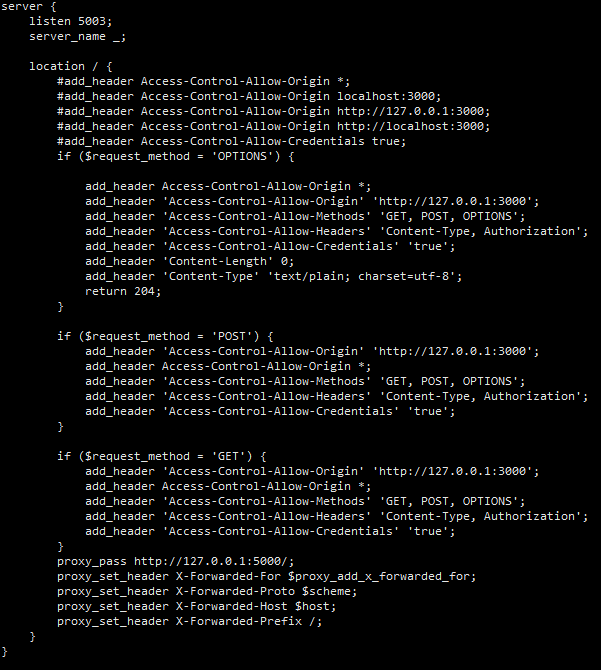
\includegraphics[width=3in]{figures/solution-nginx.png}
  \caption{Reverse Proxy server by Nginx}
  \label{fig:reversesolution}
  \end{figure}

\subsection{Interface adjustment and troubleshooting, communication between front-end and back-end}
During the software engineering process, effective communication between front-end and back-end teams is critical to successfully tuning interfaces. Postman is a powerful tool that can play a key role in this process. The following are the steps to use Postman to communicate with the back-end interface, adjust the interface, and troubleshoot based on the software engineering process:
\subsubsection{Define and understand interface specifications}
\begin{itemize}
  \item Requirements analysis: In the early stages of development, our front-end and back-end teams jointly reviewed functional requirements and clarify the purpose and expected behavior of the interface.
  \item Interface documentation: Backend teams created detailed interface documentation, including endpoint URLs, request methods (GET, POST, etc.), request parameters, expected response formats, and status codes, as shown in Fig.\ref{fig:interfacespec}.
  \item Review and feedback: Our front-end team reviewed these documents and ask questions or request changes.
\end{itemize}

\begin{figure}[h]
  \centering
  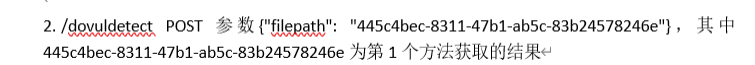
\includegraphics[width=3in]{figures/solution-interspec.png}
  \caption{Interface documentation}
  \label{fig:interfacespec}
  \end{figure}

\subsubsection{Use Postman(Fig.\ref{fig:postman}) for interface testing}
\begin{itemize}
  \item Write a request: According to the interface document, set the URL, method, header, parameters, etc. of the request.
  \item Send a request: Execute the request and observe the response. Check whether the response status code, data structure and data content are as expected.
\end{itemize}

\begin{figure}[!t]
  \centering
  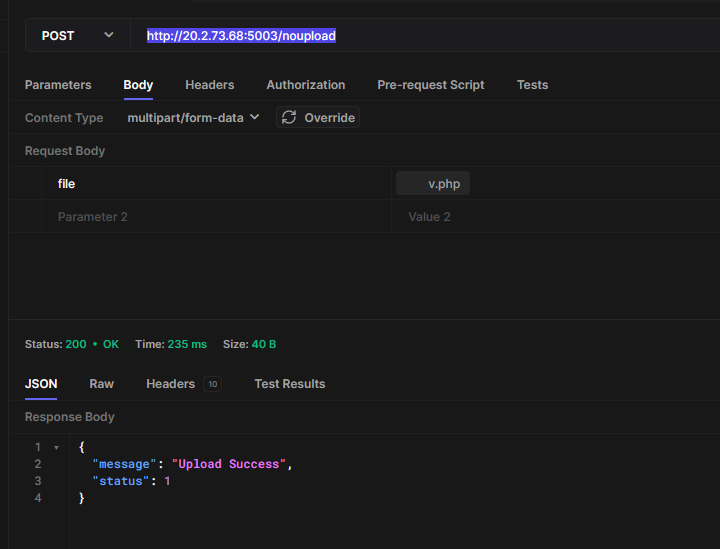
\includegraphics[width=3in]{figures/solution-postman.png}
  \caption{Postman for interface testing}
  \label{fig:postman}
  \end{figure}

\subsubsection{Interface debugging and troubleshooting}
\begin{itemize}
  \item Record and share results: Use Postman's to record and share test results with your backend team, especially when issues were discovered.
  \item Error identification: For error responses, analyze the error message or status code in the response body to determine the nature of the error.
\end{itemize}
\subsubsection{Communication and collaboration}
\begin{itemize}
  \item Feedback and modifications: Feed back the problems discovered during testing to the backend team and discuss how to modify the interface to meet needs.
  \item Update documentation: Once the interface changes, make sure to update the interface documentation to keep the documentation up-to-date.
  \item Iterative testing: Repeat testing of the modified interface to ensure that all issues have been resolved.
\end{itemize}

\begin{figure*} 
  \centering
\subfloat[\label{1a}]{%
     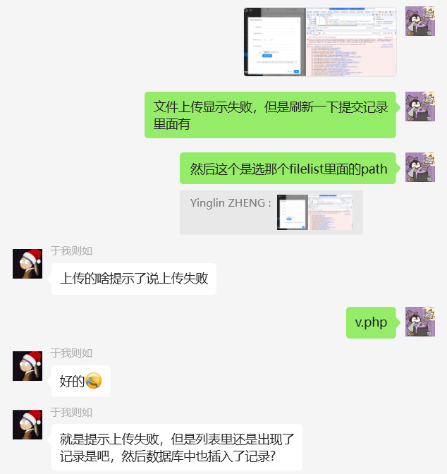
\includegraphics[height=2in,width=0.3\textwidth]{figures/collaboration1.png}}
  \hfill
\subfloat[\label{1b}]{%
      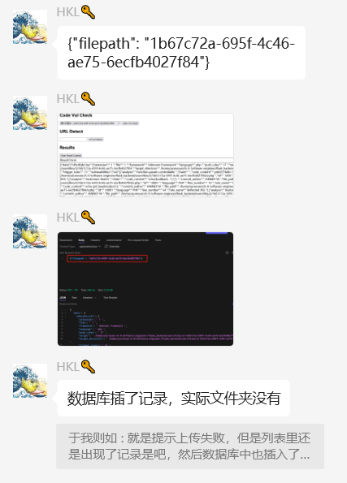
\includegraphics[height=2in,width=0.3\textwidth]{figures/collaboration2.png}}
  \hfill
\subfloat[\label{1c}]{%
      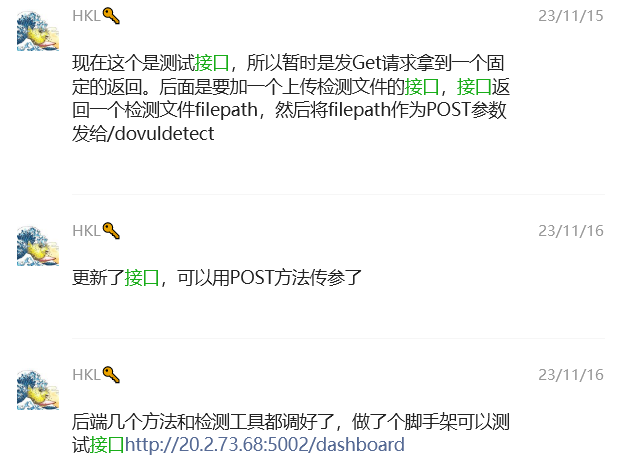
\includegraphics[height=2in,width=0.3\textwidth]{figures/collaboration3.png}}
  \hfill
  \\
\subfloat[\label{1d}]{%
      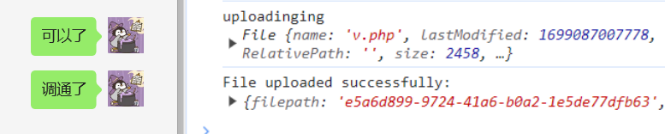
\includegraphics[height=0.8in,width=0.5\textwidth]{figures/collaboration4.png}}
\caption{(a), (b) Feed back the problems discovered during testing to the backend team and discuss how to modify the interface to meet needs.(c) Once the interface changes, make sure to update the interface documentation to keep the documentation up-to-date,(d) Iterative testing: Repeat testing of the modified interface to ensure that all issues have been resolved.}
\label{fig:collaboration} 
\end{figure*}


\subsection{Collaboration between different front-end developers}
In the software engineering process, using Git for version control and branch management is a common practice, especially in projects where multiple people collaborate. The following is the branch strategy of our front-end development team based on Git.
\subsubsection{Create a front-end branch}
Create a development branch (front-end) from the main branch. This branch contains all the latest front-end development work.
\subsubsection{Separate feature branches from the development branch}
Each developer creates his or her own branch (Yinglin-ZHENG, Xi-CHEN, etc.) from the development branch to develop assigned functional tasks or fix bugs, which ensures that development work is independent of each other and reduces conflicts.
\subsubsection{Add Readable commits and Request Review for Merge}
Developers committed their code with readable information and requested review and test from each other's, then wait for other coders to make comment, if the function is completed correctly, it can be merged into front-end branch. If there are something conflict when merge, we made a discussion between the code writers.

\subsection{Deal With JSON Response in front-end}
\subsubsection{Data interaction and analysis}
\begin{itemize}
  \item Receive JSON data: The front end receives a JSON formatted response from the back end. This is achieved by using the Fetch API and processing the response, as shown in Fig.\ref{fig:datainteana1a}.
  \item Parse JSON: The front-end application parses JSON data and converts it into JavaScript objects for further processing and display, as shown in Fig.\ref{fig:datainteana1b}.
\end{itemize}

\begin{figure} 
  \centering
\subfloat[Receive JSON data\label{fig:datainteana1a}]{%
     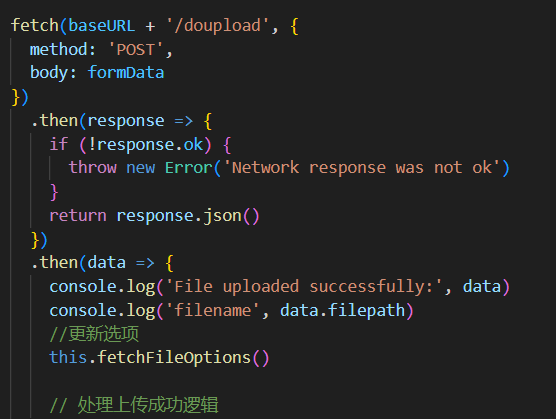
\includegraphics[height=2in,width=0.45\linewidth]{figures/json1.png}}
  \hfill
\subfloat[Parse JSON\label{fig:datainteana1b}]{%
      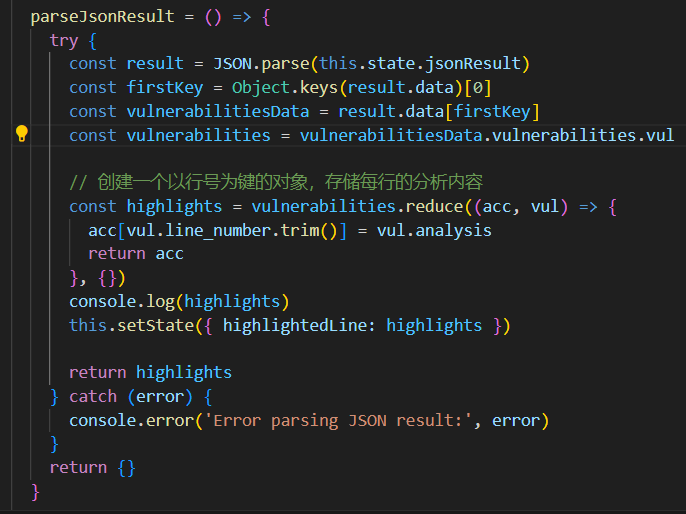
\includegraphics[height=2in,width=0.45\linewidth]{figures/json2.png}}
\caption{Data interaction and analysis}
\label{fig:datainteana} 
\end{figure}

\subsubsection{Front-end interface design}

\begin{itemize}
  \item Display code: Use appropriate HTML elements such as <pre> and <code> tags to display code, as shown in Fig.\ref{fig:displaycode}.
  \item Code highlighting: Use front-end libraries highlight.js, to implement code highlighting, as shown in Fig.\ref{fig:highlightcode}. 
\end{itemize}

\begin{figure}[!t]
  \centering
  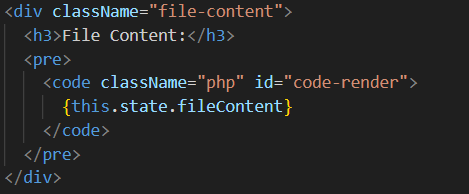
\includegraphics[width=2in]{figures/displaycode.png}
  \caption{Display code}
  \label{fig:displaycode}
  \end{figure}

\begin{figure}[!t]
  \centering
  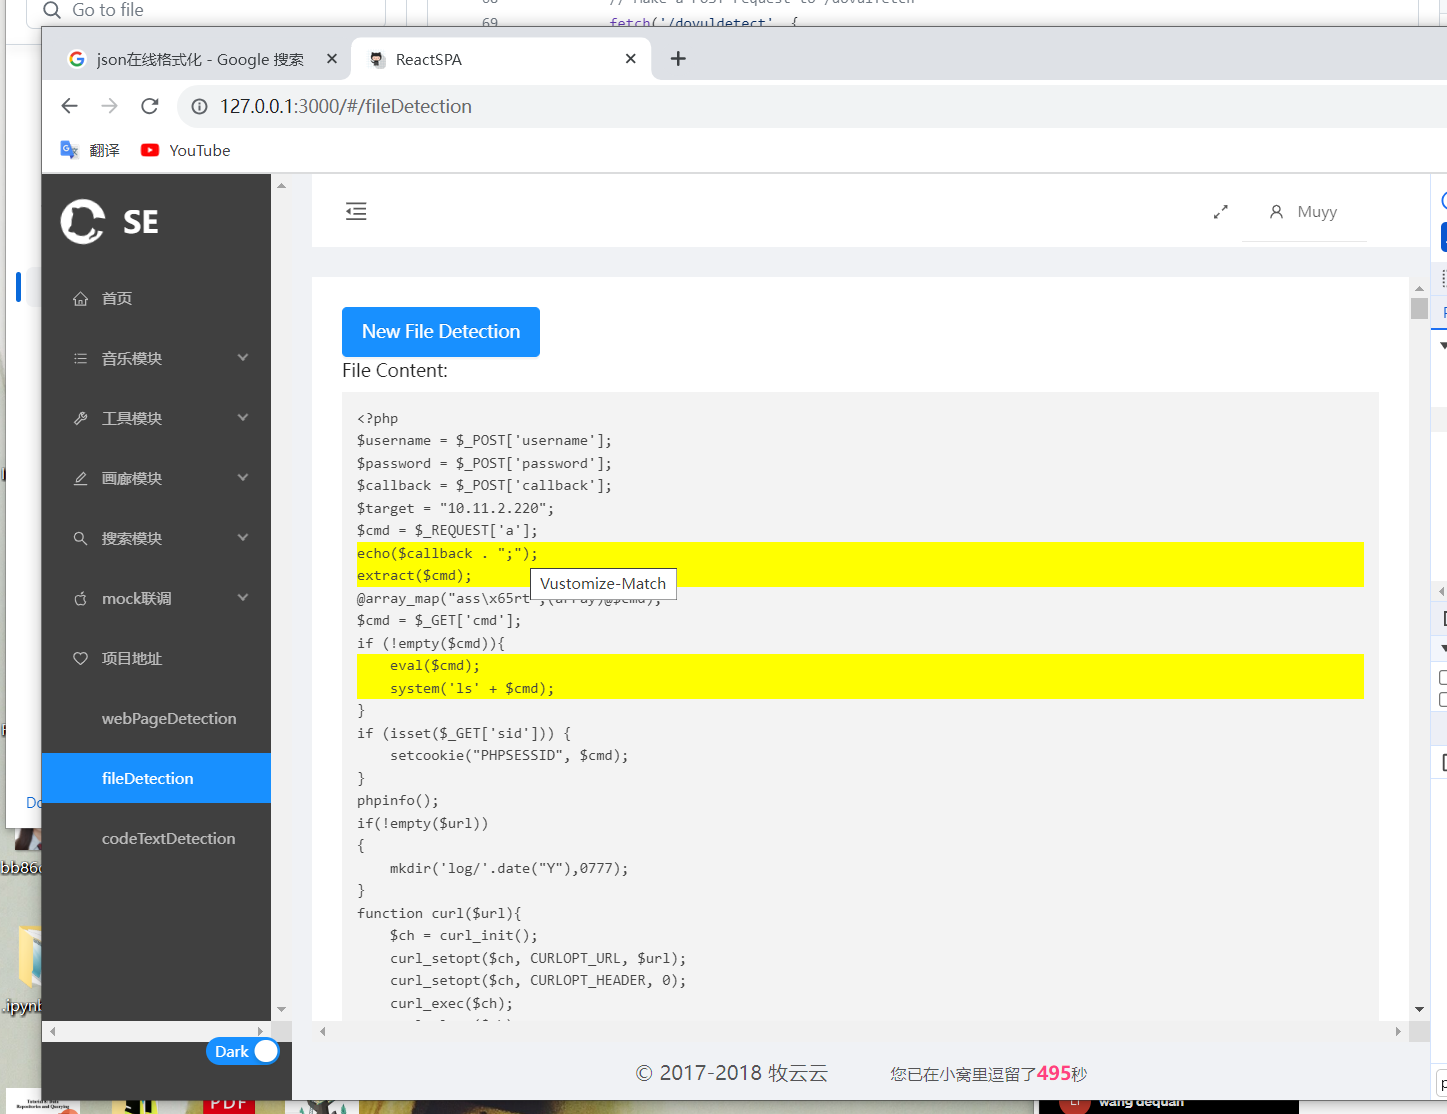
\includegraphics[width=3in]{figures/highlightcode.png}
  \caption{Code highlighting}
  \label{fig:highlightcode}
  \end{figure}

\subsubsection{Implementation of interactive functions}
\begin{itemize}
  \item Hover tip implementation: When the mouse hovers over a specific code segment, a tooltip is displayed to display the vulnerability analysis of the code segment.
  \item Correlate vulnerability data: Store vulnerability analysis metadata (e.g. using data-attributes) in each highlighted section of code for retrieval and display on hover.
\end{itemize}


\subsection{Reusable component implementation}
\subsubsection{Requirement analysis}
\begin{itemize}
  \item Functional requirements: Determine the functions that the component needs to support, such as user input, confirm/cancel buttons, close icons, etc.
  \item User interface requirements: Define the appearance of the pop-up window, including size, etc.
\end{itemize}

\subsubsection{Design}
\begin{itemize}
  \item Architecture design: designing component as an independent reusable component.
  \item Interface design: Create interface prototypes or design drawings of pop-up components.
  \item Interaction design: Plan how users interact with pop-up windows, such as handling click events.
\end{itemize}

\subsubsection{Implementation}
\begin{itemize}
  \item Create React components using antd UI style
  \item State management: Manage the display/hidden state of the componets ( such as pop-up window)
\end{itemize}

\subsubsection{Test}
\begin{itemize}
  \item Ensure that the appearance and interaction of the pop-up window meet the design requirements.
  \item Collect feedback on popup components from users or stakeholders
\end{itemize}


\vspace{1em}
\textit{Requirements: Present your solution, probably with algorithms, figures, code listing, and an example walkthrough to assist you in presenting your solution. Relate the content to each topic covered in CS5351.}

\textbf{(2-3 pages)}


\subsection{Multi-Platform}

To maximize accessibility, our tool is designed for deployment in diverse scenarios, with a focus on both user-friendly web access and a simplified GUI for desktop users. This approach aligns with the principles of usability and adaptability emphasized in software engineering.

\subsubsection{B/S-Based Application}

Our primary deployment targets a Browser/Server (B/S) architecture, providing users with a seamless and user-friendly experience. This platform-independent approach ensures that developers can easily access and utilize our tool without the need for specific operating systems or installations. This aligns with software engineering emphasis on web-based technologies and their relevance in modern software development.

\subsubsection{Desktop GUI}

Recognizing the diversity in developer preferences and environments, we also provide a straightforward Graphical User Interface (GUI) for desktop users. This option ensures that our tool caters to developers who may prefer a local installation or work within specific desktop environments. This versatility resonates with the adaptability concepts covered in software engineering.

\subsection{DevOps Integration}
\label{sol:devops}

In keeping with contemporary software engineering practices, our tool is deployed using robust DevOps practices, aligning with the DevOps principles covered in software engineering.

\subsubsection{Cloud Deployment on Microsoft Azure}

We leverage Microsoft Azure for cloud deployment, offering scalability, reliability, and a range of services that enhance the overall performance of our tool. This choice aligns with software engineering's coverage of cloud computing and its role in modern software development.

\subsubsection{Containerization with Docker}

To enhance portability and consistency across different environments, we utilize Docker for containerization. This allows our tool and its dependencies to be packaged together, ensuring that it runs consistently on various platforms. This aligns with software engineering's coverage of containerization and its impact on software deployment.

\begin{algorithm}[hbt!]
    \caption{Scalability Model}\label{alg:Scalabilitymodel}
    \begin{algorithmic}
    
    \Require $Deployment\ Definition$
  
    \State Initialization($Deployment\ Definition$) 

    \Repeat
        \State Monitoring($sys\_Status$)
        \State $New\ Definition$ $\gets$ Replica\_Calculation($sys\_Status$)
        \State Initialization($New\ Definition$) 
    \Until{$Done$}
    
    \end{algorithmic}
  \end{algorithm}

\subsubsection{Kubernetes for Scalability}

Ensuring our tool's robustness and scalability, we employ Kubernetes for container orchestration in algorithm \ref{alg:Scalabilitymodel}. This choice aligns with software engineering's exploration of scalable architectures and their significance in handling diverse workloads efficiently.

\begin{figure}[!t]
\centering

\includegraphics[width=2.5in]{figures/k8slogo.png}
\caption{Employing DevOps Techniques.}
\label{fig:k8slogo}
\end{figure}


\section{Software Process}
\noindent The 5th part is Software Process..

The Software Process section documents the team's activities throughout the project, highlighting the achievements of each sprint. Each sprint is elaborated on in two pages, capturing the essence of the tasks undertaken, challenges faced, and milestones achieved. Additionally, the section includes a burndown chart, offering a visual representation of project progress throughout its duration.


\textit{Requirements: Document the activities and the achieved of each sprint in 2 pages (a total of 2*N pages for a project with N sprints). Include the burndown chart for the whole project.}



\textbf{(each sprint in 2 pages (a total of 2*N pages for a project with N sprints))}

\section{Evaluation}
\noindent The 6th part is Evaluation...


The Evaluation section summarizes the verification and evaluation processes applied to the solution. It outlines how the team gauged the effectiveness of the tool in solving the identified code smell problems. Special attention is given to scalability considerations, comparing the results to existing tools in the software engineering landscape.


\textit{Requirements: Summarize what you have verified or evaluated your solution to have solved the problem stated in the report, and compare to the results of existing tools}

\textbf{(2-5 pages)}


\subsection{Security}
The evaluation dives into the scalability of the developed tools, exploring their performance in handling varying codebase sizes. This section utilizes equations and figures to demonstrate scalability metrics. A comparative analysis with existing tools further validates the tool's efficacy.


\subsection{Scalability}
\label{evaluate:Scalability}

Scalability is a critical aspect of our code smell detection tool, as it determines its ability to handle diverse and large-scale software projects efficiently. The evaluation involves several key components:

\subsubsection{Test Scenarios}

We conducted scalability tests across a spectrum of software projects, ranging from small-scale applications to large enterprise-level systems. This diversity ensures that our tool's performance is assessed under realistic conditions.

\subsubsection{Metrics}

To quantify scalability, we measured the tool's performance based on key metrics, including execution time, memory usage, and response time. These metrics provide insights into how well the tool handles increasing codebase sizes without significant degradation in performance.

\subsubsection{Comparison with Existing Tools}

To contextualize our results, we compared the scalability of our tool with existing code smell detection tools in the industry. This comparative analysis offers a benchmark for understanding the tool's performance relative to established solutions.

\subsubsection{Scalability Equations}

We utilized scalability equations to model the tool's performance as the size of the codebase increases. These equations help predict how the tool will scale in different scenarios and provide valuable insights for future users.

\subsubsection{Parallel Processing}

Incorporating principles covered in software engineering, our tool utilizes parallel processing techniques to enhance scalability. This involves efficiently distributing the workload across multiple processing units, mitigating bottlenecks and improving overall performance.

\subsubsection{Dynamic Scaling}

Our tool employs dynamic scaling mechanisms, adjusting resource allocation based on the size and complexity of the codebase being analyzed. This adaptive approach ensures optimal performance across a wide range of scenarios.

\subsubsection{Results and Analysis}

The scalability evaluation yielded promising results, showcasing our tool's ability to efficiently handle diverse codebases. Execution times remained within acceptable limits even as project sizes increased. Memory usage demonstrated stability, and response times were consistently low.

Comparison with existing tools highlighted the competitive scalability of our solution, positioning it as a viable option for developers working on projects of varying scales.

\subsubsection{Future Considerations}

To ensure continued scalability as software projects evolve, we outline plans for future enhancements. This includes ongoing optimization efforts, monitoring for potential bottlenecks, and incorporating feedback from users to address specific scalability challenges in real-world scenarios.



\section{Conclusion}
\noindent The 7th part is Conclusion...

The Conclusion section provides a concise recap of the main achievements, encompassing the software development process, activities, techniques, deliverables, the tool itself, and noteworthy best practices. Additionally, the team outlines areas for future work, indicating the potential evolution of the tools and any further enhancements planned.

\textit{Requirements: Recap the main achievement (process, activities, techniques, deliverables, tool, people, and best practice) and future work.}

\textbf{(about 1 page)}


\bibliographystyle{ieeetr} 
\bibliography{refs} % Entries are in the refs.bib file

\vspace{-5 mm}
\begin{IEEEbiography}[{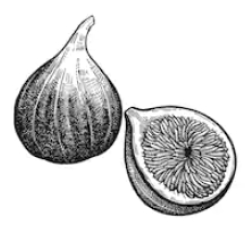
\includegraphics[width=1in,height=1.25in,clip,keepaspectratio]{figures/fig1.png}}]{Biography} According to the requirements that in the Project PPT. Biography is required. Such AS:\\
1. The bio of each student including the declaration of the contribution of the student.\\
2. Present a bio of each student. Who you are, your background, technical ideas, current interests, etc. Give a \textcolor{BurntOrange}{self-reflection} on the work done by you. \textcolor{BurntOrange}{State and justify your contribution} to the project.


\end{IEEEbiography}

\input{private/bio}

\end{document}


